%% LyX 1.6.7 created this file.  For more info, see http://www.lyx.org/.
%% Do not edit unless you really know what you are doing.
\documentclass[english]{article}
\usepackage[T1]{fontenc}
\usepackage[latin9]{inputenc}
\usepackage[letterpaper]{geometry}
\geometry{verbose,tmargin=1in,bmargin=1in,lmargin=1in,rmargin=1in}
\setcounter{tocdepth}{1}
\usepackage{babel}

\usepackage{amsmath}
\usepackage{graphicx}
\usepackage{amssymb}
\usepackage[unicode=true, pdfusetitle,
 bookmarks=true,bookmarksnumbered=false,bookmarksopen=false,
 breaklinks=true,pdfborder={0 0 0},backref=false,colorlinks=false]
 {hyperref}

\makeatletter

%%%%%%%%%%%%%%%%%%%%%%%%%%%%%% LyX specific LaTeX commands.
\providecommand{\LyX}{L\kern-.1667em\lower.25em\hbox{Y}\kern-.125emX\@}
%% Special footnote code from the package 'stblftnt.sty'
%% Author: Robin Fairbairns -- Last revised Dec 13 1996
\let\SF@@footnote\footnote
\def\footnote{\ifx\protect\@typeset@protect
    \expandafter\SF@@footnote
  \else
    \expandafter\SF@gobble@opt
  \fi
}
\expandafter\def\csname SF@gobble@opt \endcsname{\@ifnextchar[%]
  \SF@gobble@twobracket
  \@gobble
}
\edef\SF@gobble@opt{\noexpand\protect
  \expandafter\noexpand\csname SF@gobble@opt \endcsname}
\def\SF@gobble@twobracket[#1]#2{}
%% Because html converters don't know tabularnewline
\providecommand{\tabularnewline}{\\}

\makeatother

\begin{document}

\title{Theory of computation: notes for UIC qual%
\thanks{This work is licensed under a \underbar{\protect\href{http://creativecommons.org/licenses/by-nc-sa/3.0}{Creative Commons Attribution-NonCommercial-ShareAlike 3.0 Unported License}}.%
}}


\author{Gugo}

\maketitle

\subsection*{Disclaimer}

These notes have been prepared with the \textbf{only} purpose to help
me pass the Computer Science qualifiying exam at the University of
Illinois at Chicago. They are distributed as they are (including errors,
typos, omissions, etc.) to help other students pass this exam (and
possibly relieving them from part of the pain associated with such
a process). I take \textbf{no responsibility} for the material contained
in these notes (which means that you can't sue me if you don't pass
the qual!) Moreover, this pdf version is distributed together with
the original \LaTeX{} (and \LyX{}) sources hoping that someone else
will improve and correct them. I mean in absolute no way to violate
copyrights and/or take credit stealing the work of others. The ideas
contained in these pages are \textbf{not mine} but I've just aggregated
information scattered all over the internet.


\subsection*{Strongly suggested book}

Before you even start reading this notes, do yourself a favor and
go buy Michael Sipser's book. (\href{http://www-math.mit.edu/~sipser/book.html}{http://www-math.mit.edu/$\sim$sipser/book.html})
It is crispy clear and beautifully written and prepared. All people
that studied on this book passed the exam! :)

\tableofcontents{}


\section{Regular Languages}


\subsection{DFA}


\paragraph{Formal definition}

A \emph{finite automaton} is a 5-uple $(Q,\Sigma,\delta,q_{0},F$),
where 
\begin{enumerate}
\item $Q$ is a finite set called the \emph{states},
\item $\Sigma$ is a finite set called the \emph{alphabet},
\item $\delta:Q\times\Sigma\rightarrow Q$ is the \emph{transition function},
\item $q_{0}\in Q$ is the \emph{start state}, and
\item $F\subseteq Q$ is the \emph{set of accept states}.
\end{enumerate}

\paragraph{Formal definition of computation}

Let $M=(Q,\Sigma,\delta,q_{0},F)$ be a finite automaton and let $w=w_{1}w_{2}\dots w_{n}$
be a string where each $w_{i}$ is a member of the alphabet $\Sigma$.
Then $M$ accepts $w$ if a sequence of states $r_{0},r_{1},\dots,r_{n}$
in $Q$ exists with three conditions:
\begin{enumerate}
\item $r_{0}=q_{0}$,
\item $\delta(r_{i},w_{i+1})=r_{i+1}$ for $i=0,\dots,n-1$ and
\item $r_{n}\in F$.
\end{enumerate}
We say $M$ recognizes language $A$ if $A=\{w|M\, accepts\, w\}$.


\paragraph{Facts}
\begin{itemize}
\item If $A$ is the set of all strings that the machine $M$ accepts, we
say that \emph{$A$ is the language of machine $M$} and write $L(M)=A$.
We say that \emph{$M$ recognizes $A$} or that \emph{$M$ accepts
$A$}%
\footnote{Recognize is preferred because accepting may also refer to strings%
}.
\item A machine may accept several strings, but it always recognizes \emph{only
one language}. 
\item A language is \emph{regular} if some finite automaton recognizes it.
\item If the machine accepts no strings, it still recognizes one language,
that is the empty language $\emptyset$.
\item In order for a DFA to accept the empty string $\varepsilon$, the
start state must also be an accept state.
\end{itemize}

\subsection{NFA}


\paragraph{Formal definition}

A \emph{nondeterministic finite automaton} is a 5-uple $(Q,\Sigma,\delta,q_{0},F$),
where 
\begin{enumerate}
\item $Q$ is a finite set called the \emph{states},
\item $\Sigma$ is a finite set called the \emph{alphabet},
\item $\delta:Q\times\Sigma_{\varepsilon}\rightarrow\mathcal{P}(Q)$ is
the \emph{transition function},%
\footnote{Where $\Sigma_{\varepsilon}=\{\Sigma\cup\{\varepsilon\}\}$ and $\{\{\emptyset\},\{Q\}\}\in\mathcal{P}(Q)$.
Note that $\varepsilon$ indicates the empty string of length 0. Note
also how $L_{A}=\emptyset\neq L_{B}=\{\varepsilon\}$.%
}
\item $q_{0}\in Q$ is the \emph{start state}, and
\item $F\subseteq Q$ is the \emph{set of accept states}.
\end{enumerate}

\paragraph{Formal definition of computation}

Let $N=(Q,\Sigma,\delta,q_{0},F)$ be an NFA and $w$ a string over
the alphabet $\Sigma$. Then $N$ accepts $w$ if we can write $w=y_{1}y_{2}\dots y_{m}$
where each $y_{i}$ is a member of $\Sigma_{\varepsilon}$ and a sequence
of states $r_{0},r_{1},\dots,r_{n}$ in $Q$ exists with three conditions:
\begin{enumerate}
\item $r_{0}=q_{0}$,
\item $r_{i+1}\in\delta(r_{i},y_{i+1})$ for $i=0,\dots,m-1$ and
\item $r_{m}\in F$.
\end{enumerate}

\subsection{Equivalence of DFA and NFA}

The following procedure converts a NFA $N=(Q,\Sigma,\delta,q_{0},F)$
to the equivalent DFA $N'=(Q',\Sigma,\delta',q'_{0},F')$.
\begin{enumerate}
\item $Q'=\mathcal{P}(Q)$; (which means that usually the DFA is much larger
than the corresponding NFA!)
\item For $R\in Q'$ and $a\in\Sigma$ let $\delta'(R,a)=\underset{r\in R}{\bigcup}\delta(r,a)$;
(all states reachable from the states in $R$ with input $a$)
\item $q'_{0}=\{q_{o}\}$; (same start state)
\item $F'=\{R\in Q'|R\text{ contains an accept state of }N\}$\end{enumerate}
\begin{itemize}
\item If there are $\varepsilon$ arrows we need to define $E(R)=\{q|q\text{\,\ can be reched from \ensuremath{R}by traveling along 0 or more \ensuremath{\varepsilon}arrows}\}$
(called $\varepsilon$-closure) and modify points 3 and 4:


3. $\delta'(R,a)=\{q\in Q|q\in E(\delta(r,a))\, for\, some\, r\in R\}$
(same as before but all the reachable with an $\varepsilon$ arrow)

4. $q'_{0}=E(\{q_{o}\})$; (same start state and all the ones reachable
with an $\varepsilon$ arrow)

\item It is \emph{very useful} to calculate $E$ for all states before starting
the conversion procedure
\item We send a state $q$ on the $\emptyset$ state on input $a$ only
if $\delta(q,a)=\emptyset$. This represents the stuck reject. Sink
state that guarantees rejection.
\item To go from a DFA to the equivalent NFA no further action is needed
since DFAs are a particular case of NFAs.
\end{itemize}
In practice just start from the start state and compute $\delta$
only for all possible inputs and continue until no new states are
added.


\subsection{Closure automata construction%
\footnote{See pictures p. 59, 61, 62 of Sipser's book%
} }
\begin{itemize}
\item Union automata ($N_{1}\cup N_{2}$): new start state with two $\varepsilon$
arrows entering the start states of $N_{1}$ and $N_{2}$ respectively.
\item Concatenation automata ($N_{1}\cdot N_{2}$): $\varepsilon$ arrows
exiting the accept states of $N_{1}$ and entering the start state
of $N_{2}$.
\item Star automata ($N_{1}^{*}$): new start/end state with an $\varepsilon$
arrow entering the old start state%
\footnote{This is done to avoid recognition of other undesired strings other
than $\varepsilon$.%
} and $\varepsilon$ arrows connecting the accept states with the old
start state.
\end{itemize}

\subsection{Regular Expressions}

We say that $R$ is a \emph{regular expression} if $R$ is
\begin{enumerate}
\item $a$ for some $a\in\Sigma$,
\item $\varepsilon$,
\item $\emptyset$,
\item $(R_{1}\cup R_{2})$, where $R_{1}$ and $R_{2}$ are regular expressions,
\item $(R_{1}\cdot R_{2})$, where $R_{1}$ and $R_{2}$ are regular expressions,
or
\item $(R_{1}^{*})$, where $R_{1}$ is a regular expression.
\end{enumerate}

\subsubsection{Facts:}
\begin{enumerate}
\item We can write $R_{1}\cup R_{2}$ also as $R_{1}|R_{2}$
\item $R^{+}=RR^{*}$
\item $R\cup\emptyset=R$
\item $R\cdot\varepsilon=R$
\item $R\cdot\emptyset=\emptyset$
\item $\emptyset^{*}=\{\varepsilon\}$
\end{enumerate}
A language is regular if and only if some regular expression describes
it.


\subsubsection{Conversion from R.E. to NFA (if) }

We just consider the 6 points in the definition of regular expression:
\begin{enumerate}
\item Two states (start and accept) connected by an $a$ arrow
\item One state: start and accept at the same time
\item One state: start with no accept
\item $R=R_{1}\cup R_{2}$%
\footnote{See pictures p.67 of Sipser's Book for this last three points.%
}
\item $R=R_{1}\cdot R_{2}$
\item $R=R_{1}^{*}$
\end{enumerate}

\subsubsection{Conversion from DFA to R.E. (only if) }
\begin{enumerate}
\item If we have a NFA we need first to convert it to a DFA.
\item Convert the DFA $M$ into a GNFA $G$:

\begin{enumerate}
\item Add a new start state $s$ with an $\varepsilon$ arrow to the old
start state and a new accept state $a$ with $\varepsilon$ arrows
from the old accept states.
\item If any arrows have multiple labels (e.g. $\delta(q_{i},a)=\delta(q_{i},b)=q_{j}$)
replace them with a single arrow whose label is the union of the previous
labels.
\end{enumerate}
\item We choose a state ($q_{rip}$) of $G$ at the time and we eliminate
it obtaining a new GNFA $G'$:

\begin{enumerate}
\item $Q'=Q-\{q_{rip}\}$
\item For \emph{every} pair $q_{i}$ and $q_{j}$ such that $q_{i}\in Q'-q_{acc}$
and $q_{j}\in Q'-q_{start}$, $\delta'(q_{i},q_{j})=(R_{1})(R_{2})^{*}(R_{3})\cup(R_{4})$
where $R_{1}=(q_{i},q_{rip})$, $R_{2}=(q_{rip},q_{rip})$, $R_{3}=\delta(q_{rip},q_{j})$and
$R_{4}=\delta(q_{i},q_{j})$ and where $q_{i}\in Q'-q_{acc}$ and
$q_{j}\in Q'-q_{start}$.
\end{enumerate}
\item Once we have only $s$ and $a$ the label of $\delta(s,a)$ is the
regular expression
\end{enumerate}

\section{Context Free Languages}

A \emph{context-free grammar} is a 4-tuple ($V,\Sigma,R,S)$, where
\begin{enumerate}
\item $V$ is a finite set called the \emph{variables},
\item $\Sigma$ is a finite set, disjoint from $V$, called the \emph{terminals},
\item $R$ is a finite set of \emph{rules}, with each rule being a variable
and a string of variables and terminals, and
\item $S\in V$ is the \emph{start variable}.
\end{enumerate}
If $u,v$ and $w$ are strings of variables and terminals, and $A\rightarrow w$
is a rule of the grammar, we say that $uAv$ \emph{yields} $uwv$,
written $A\Rightarrow uwv$. 

Say $u$ \emph{derives} $v$, written $u\Rightarrow v$, if $u=v$
or if a sequence $u_{1},u_{2},\ldots,u_{k}$ exists for $k\geq0$
and $u\Rightarrow u_{1}\Rightarrow u_{2}\Rightarrow\ldots\Rightarrow u_{k}\Rightarrow v$. 

The \emph{language} of the grammar is $\{w\in\Sigma^{*}|S\overset{*}{\Rightarrow}w\}$.


\subsection{Ambiguity}
\begin{itemize}
\item A derivation of a string $w$ in a grammar $G$ is a \emph{leftmost
derivation} if at every step the leftmost remaining variable is the
one being replaced. (Two derivations may differ merely in the order
in which they replace variables yet not in their overall structure!)
\item A string is derived \emph{ambiguously} in a CFG $G$ if it has two
or more different leftmost derivations. Grammar $G$ is \emph{ambiguous}
if it generates some string ambiguously.
\item Some CFLs, however, can be generated only by ambiguous grammars: these
languages are called inherently ambiguous.
\end{itemize}

\subsection{Chomsky normal form}

A CFG is in Chomsky normal for if every rule is of the form 
\begin{enumerate}
\item $A\rightarrow BC$
\item $A\rightarrow a$
\end{enumerate}
where $a$ is any terminal and $A$, $B$ and $C$ are any variable
- except that B and C may not be the start variable. In addition we
permit the rule $S\rightarrow\varepsilon$, where $S$ is the start
variable.
\begin{itemize}
\item Any CFL is generated by a CFG in Chomsky normal form
\item Any string $w$ such that $|w|=n$ can be derived with $\frac{n}{2}$
derivations
\item Every regular language is context free
\item CNF is useful when working with grammar related algorithms
\end{itemize}

\subsection{Push Down Automata (PDA)}
\begin{itemize}
\item A language is context free if and only if some push down automaton
recognizes it.
\end{itemize}
Not asked in the theory part but useful for compilers!!!


\section{Turing machines}


\paragraph{Formal definition}

A \emph{Turing machine} is a 7-uple $(Q,\Sigma,\Gamma,\delta,q_{0},q_{accept},q_{reject}$),
where $Q,\Sigma,\Gamma$ are all finite sets and
\begin{enumerate}
\item $Q$ is the set of \emph{states},
\item $\Sigma$ is the \emph{input alphabet} not containing the \emph{blank
symbol} $\sqcup$,
\item $\Gamma$ is the \emph{tape alphabet} where $\sqcup\in\Gamma$ and
$\Sigma\subseteq\Gamma$,
\item $\delta:Q\times\Gamma\rightarrow Q\times\Gamma\times\{L,R\}$ is the
transition function,
\item $q_{0}\in Q$ is the start state,
\item $q_{accept}\in Q$ is the accept state, and
\item $q_{reject}\in Q$is the reject state, where $q_{accept}\neq q_{reject}$.
\end{enumerate}

\paragraph{Computation }

We define a \emph{configuration} of a TM as a setting of the state,
the current tape content and the current head location. We usually
represent them as a string $uqv$ where $q$ is a state, $uv$ is
the current tape content and the head location is the first symbol
of $v$. The tape contains only blanks following the last character
of $v$.
\begin{itemize}
\item The \emph{start configuration} of $M$ on input $w$ is $q_{0}w$. 
\item In an \emph{accepting configuration} the state of the configuration
is $q_{accept}$. 
\item In a \emph{rejecting configuration} the state of the configuration
is $q_{reject}$. 
\item Accepting and rejecting configurations are \emph{halting configurations}
and \underbar{do not} yield further configurations.
\item A Turing machine $M$ accepts input $w$ if a sequence of configurations
$C_{1}C_{2},\ldots,C_{k}$ exists, where

\begin{itemize}
\item $C_{1}$ is the start configuration of $M$ on input $w$,
\item each $C_{i}$ yields $C_{i+1}$
\item $C_{k}$ is an accepting configuration.
\end{itemize}
\end{itemize}

\paragraph{Facts}
\begin{itemize}
\item When we start a TM, three outcomes are possible: accept, reject or
loop (the TM doesn't halt)
\item We call a language \emph{Turing-recognizable} (or recursively enumerable)
if some Turing machine recognizes it. I can enumerate all the {}``yes''
instances (strings that are accepted)
\item Turing machines that halt on every input are called \emph{deciders}
because they always make a decision to accept or reject.
\item We call a language \emph{Turing-decidable} (or recursive) if some
Turing machine decides it. Every decidable language is Turing-recognizable.
\end{itemize}

\subsection{Variants of Turing machine}

Every \emph{multitape} Turing machine has an equivalent single-tape
Turing machine.

Every \emph{nondeterministic} Turing machine has an equivalent deterministic
Turing machine. Which means that nondeterminism does not affect the
power of the Turing machine model.


\subsection{Church-Turing thesis}

We choose to represent various computational problems by languages;
which means we reduce algorithms (and problems) to languages that
can or cannot be accepted by a Turing machine. If such a TM is a decider
then the language (and therefore the problem) is decidable. 


\section{Decidability}


\subsection{Decidable languages}
\begin{itemize}
\item $A_{DFA}=\{\left\langle B,w\right\rangle |B\text{ is a DFA that accepts input string }w\}$
is a decidable language. $A_{DFA}$ represents the problem of testing
whether a particular deterministic finite automaton $B$ accepts a
given string $w$: doing this is the same problem of testing whether
$\left\langle B,w\right\rangle $ is a member of the language $A_{DFA}$.
(To prove this just simulate $B$ on $M$ and if the simulation ends
in an accept state, accept, otherwise, reject. The TM will terminate
because $w$ is finite)
\item $A_{NFA}=\{\left\langle B,w\right\rangle |B\text{ is a NFA that accepts input string }w\}$
is a decidable language. (Proof: convert NFA to DFA)
\item $A_{REX}=\{\left\langle R,w\right\rangle |R\text{ is a regular expression that generates string }w\}$
is a decidable language. (Proof: convert REX to DFA)
\item $E_{DFA}=\{\left\langle A\right\rangle |A\text{ is a DFA and }L(A)=\emptyset\}$
is a decidable language. (Proof: Mark the states of $A$ following
the arrows and starting from the start state; if no accept state is
marked, accept, otherwise, reject. The TM will terminate because $|Q_{A}|$
is finite.)
\item $EQ_{DFA}=\{\left\langle A,B\right\rangle |A\text{ and }B\text{ are DFAs and }L(A)=L(B)\}$
is a decidable language. (Proof: construct $L(C)=L(A)\otimes L(B)$
and test $E_{DFA}(C)$.)
\item $A_{CFG}=\{\left\langle G,w\right\rangle |G\text{ is a CFG that generates string }w\}$
is a decidable language. (Proof: Convert grammar in Chomsky normal
form, list all derivations with length $2|w|-1$ steps, if any of
these derivations generate $w$, accept, otherwise, reject. TM will
terminate because the number of productions of length $2|w|-1$ steps
is finite.)
\item $E_{CFG}=\{\left\langle G\right\rangle |G\text{ is a CFG and }L(G)=\emptyset\}$
is a decidable language. (Proof: Mark all terminals, mark any variable
$A$ where $G$ has a rule $A\rightarrow U_{1}U_{2}\ldots U_{k}$
and each symbol $U_{1}U_{2}\ldots U_{k}$ has already been marked,
if $S$ is not marked accept, otherwise, reject. TM will terminate
because number of variables in $G$ is finite.)
\item $EQ_{CFG}$ is \emph{undecidable}! (Because CFG are not closed w.r.t.
intersection and complement)
\end{itemize}
Every context free language is decidable. This implies $\text{regular}\subseteq\text{context free}\subseteq\text{decidable}\subseteq\text{Touring recognizable}$.


\subsection{The halting problem}

$A_{TM}=\{\left\langle M,w\right\rangle |M\text{ is a TM and M accepts input string }w\}$
is undecidable.

Proof is by contradiction using diagonalization. Suppose $H$ is a
decider for $A_{TM}$ that, on input $\left\langle M,w\right\rangle $,
accepts if $M$ accepts $w$, and rejects if $M$ does not accept
$w$ (including loops). We can define another TM $D$ with$H$ as
a subroutine that, on input $\left\langle M\right\rangle $, runs
$H(M,\left\langle M\right\rangle )$ and outputs the opposite of what
$H$ outputs; that is, if $H$ accepts, reject and if $H$ rejects,
accept. Run $D(\left\langle D\right\rangle )$ and observe that no
matter what $D$ does, it is forced to do the opposite, which is obviously
a contradiction. Thus neither $M$ nor $H$ can exist.
\begin{itemize}
\item $A_{TM}$ is Turing-recognizable (we can simulate $\left\langle M,w\right\rangle $
on a Turing machine $U$ that accepts if $M$ accepts, rejects if
$M$ rejects and loops if $M$ loops).
\item Some languages are not Turing recognizable. (We prove this by showing
that the set of all Turing machines is countable while the set of
all languages is uncountable) This means that there are some languages
which not only can't be decided by a Turing machine but can't even
be recognized by it.
\item A language (only one, not the class!) is \emph{co-Turing-recognizable}
if it is the complement of a Turing-recognizable language. Co-RE languages
are the ones for which I can enumerate all the NO instances (strings
not accepted).
\item A language (only one, not the class!) is decidable if and only if
it is both Turing-recognizable and co-Turing-recognizable. $\text{R}=\text{RE}\cap\text{co-RE}$.
\item $\overline{A_{TM}}$ is not Turing-recognizable.
\end{itemize}

\section{Reducibility}

A \emph{reduction} is a way of converting one problem to another problem
in such a way that a solution to the second problem can be used to
solve the first problem.

As a rule of thumb, every time an unknown $A$ can be reduced to a
more specific $B$ we can say $A$ gets the same more specific properties
of $B$. Vice-versa, whenever $A$ can be reduced to an unknown $B$
the only thing we can assert is that \textbf{$B$} has the same general
properties of $A$.


\subsection{Mapping reducibility}

A function $f:\Sigma^{*}\rightarrow\Sigma^{*}$ is a \emph{computable
function} if some Turing machine $M$, on every input $w$, halts
with just $f(w)$ on its tape.

Language $A$ is \emph{mapping reducible} to language $B$, written
$A\leq_{m}B$, if there is a computable function $f:\Sigma^{*}\rightarrow\Sigma^{*}$,
where for every $w$, $w\in A\iff f(w)\in B$. The function $f$ is
called \emph{reduction} of $A$ to $B$.


\subsubsection{Facts}
\begin{itemize}
\item Note how the previous definition also implies $w\notin A\iff f(w)\notin B$
that is $\bar{A}\leq_{m}\bar{B}$.
\item If $A\leq_{m}B$ and $B$ is decidable, then $A$ is decidable. (Proof:
we have a decider $M$ for $B$. Therefore we can specify a decider
for $A$ that first computes $f(w)$ and then runs $M$ on input $f(w)$
and outputs whatever $M$ outputs)
\item If $A\leq_{m}B$ and $A$ is undecidable, then $B$ is undecidable.
(Proof: corollary of the previous one)
\item If $A\leq_{m}B$ and $B$ is Turing-recognizable, then $A$ is Turing-recognizable.
(Proof: same as before)
\item If $A\leq_{m}B$ and $A$ is not Turing-recognizable, then $B$ is
not Turing-recognizable. (Proof: corollary of the previous one) Since
we know that $\overline{A_{TM}}$is not Turing recognizable we often
let $A$ be $\overline{A_{TM}}$ so that, to show $B$ is not Turing-recognizable,
we just need to prove $A_{TM}\leq_{m}\bar{B}$ (which is equivalent
to $\overline{A_{TM}}\leq_{m}B$.
\end{itemize}

\subsection{Undecidable problems}
\begin{itemize}
\item $HALT_{TM}$ is undecidable. Proof of this theorem illustrates the
general technique to prove undecidability! By contradiction we assume
$HALT_{TM}$ is decidable and we show that $A_{TM}$ is reducible
to $HALT_{TM}$ which will imply that $A_{TM}$ is decidable too,
which is clearly a contradiction.
\item $E_{TM}=\{\langle M\rangle|M\text{ is a TM and }L(M)=\emptyset\}$
is undecidable. (Proof: we assume that $E_{TM}$ is decidable and
then we show that this yields to the decidability of $A_{TM}$)
\item $EQ_{TM}=\{\langle M_{1},M_{2}\rangle|M_{1}\text{ and }M_{2}\text{ are TMs and }L(M_{1})=L(M_{2})\}$
is undecidable. (Proof: show that $E_{TM}$ is reducible to $EQ_{TM}$
and, therefore, if $EQ_{TM}$ were decidable, $E_{TM}$ also would
be decidable. )
\item $REGULAR_{TM}=\{\langle M\rangle|M\text{ is a TM and }L(M)\text{ is a regular language}\}$
is undecidable. 
\item \emph{Rice's theorem}. Let $P$ be any nontrivial property of the
language of a Turing Machine. The problem of determining whether a
given Turing Machine's language has property $P$ is undecidable.
\item $A_{LBA}=\{\langle M,w\rangle|M\text{ is a LBA that accepts string }w\}$
is decidable. A\emph{ linear bounded automaton }(LBA) is a restricted
type of Turing machine wherein the tape head isn't permitted to move
off the portion of the tape containing the input. This automata recognizes
languages that are Type-1 in the Chomsky classification. (Proof: the
reason why the problem is decidable is that such and automata can
have only a limited number of configurations when string of length
$n$ is the input, which means such an automata can be simulated on
a TM which will be able to recognize when a loop occurs, thanks to
the finite amount of configurations)
\end{itemize}

\section{Complexity}

Let $M$ be a deterministic TM that halts on all inputs. The running
time or time complexity of $M$ is the function $f:\mathbb{N}\rightarrow\mathbb{N}$,
where $f(n)$ is the maximum number of steps that a $M$ uses on any
input of length $n$. If $f(n)$ is the running time of $M$, we say
that $M$ runs in time $f(n)$ and that $M$ is an $f(n)$ time TM.

Let $f$ and $g$ be functions $f,g:\mathbb{N}\rightarrow\mathbb{R}^{+}$.
Say that $f(n)=O(g(n))$ if positive integers $c$ and $n_{0}$ exists
such that for every integer $n\geq n_{0}$, $f(n)\leq cg(n)$. $ $Using
the asymptotic notation allows us to omit details of the machine description
that affect the running time by at most a constant factor.


\subsection{Complexity relationships among models}

Let $t:\mathbb{N}\rightarrow\mathbb{R}^{+}$ be a function. Define
the \emph{time complexity class}, $TIME(t(n))$, to be the collection
of all languages that are decidable by an $O(t(n))$ Turing Machine.

Let $t(n)$ be a function, where $t(n)\geq n$. Then every $t(n)$
time multitape Turing machine has an equivalent $O(t^{2}(n))$ time
single-tape Turing machine.

Let $N$ be a nondeterministic Turing machine that is a decider. The
running time of $N$ is the function $f:\mathbb{N}\rightarrow\mathbb{N}$,
where $f(n)$ it the maximum number of steps that $N$uses on any
branch of its computation on any input of length $n$.

Let $t(n)$ be a function, where $t(n)\geq n$. Then every $t(n)$
time nondeterministic Turing machine has an equivalent $2^{O(t(n))}$
time deterministic single-tape Turing machine. (Which means nondeterministic
machines are exponentially quicker than deterministic TMs!)


\subsection{The class P}

P is the class of languages that are decidable in polynomial time
on a deterministic single-tape Turing machine. In other words,\[
P=\underset{k}{\bigcup}TIME(n^{k})\]


P roughly corresponds to the class of problems realistically solvable
on a computer. All reasonable deterministic models are polynomially
equivalent


\subsubsection{Examples of problems in P}

When we analyze an algorithm to show that it runs in polynomial time,
we need to do two things. First, we need to give a polynomial upper
bound on the number of stages that the algorithm uses when it runs
on an input of length $n$. Then, we have to examine the individual
stages in the description of the algorithm to be sure that each stage
can be implemented in polynomial time on a reasonable deterministic
model. Also, we need to make sure that a reasonable encoding method
for the problem is used where by {}``reasonable method'' we mean
one that allows for polynomial time encoding and decoding of objects
into natural internal representation.
\begin{itemize}
\item $PATH=\{\langle G,s,t\rangle|G\text{ is a directed graph that has a directed path from }s\text{ to }t\}$
is P. (Proof: run BFS/DFS starting from $s$)
\item $RELPRIME=\{\langle x,y\rangle|x\text{ and }y\text{ are relatively prime}\}$
is P. (i.e. 1 is the largest number that divides both)
\item Every CFL (and therefore every CFG) is a member of P. (Proof: we already
proved that $A_{CFG}$ is decidable, we just need to show that the
algorithm used in that proof runs in polynomial time, unfortunately
it doesn't so we need to devise a new one using dynamic programming)
\end{itemize}

\subsection{The class NP}

A \emph{verifier} for a language $A$ is an algorithm $V$, where
$A=\{w|V\, accepts\,\langle w,c\rangle\, for\, some\, string\, c\}$.
We measure the running time of a verifier only in terms of the length
of $w$ so a \emph{polynomial time verifier} runs polynomial time
in the length of $w$. 

A language $A$ is \emph{polynomial time verifiable} if it has a polynomial
time verifier.

A verifier uses additional information, represented by the symbol
$c$ in the previous definition, to verify that string $w$ is a member
of $A$. This information is called a \emph{certificate} or \emph{proof}.

NP is the class of languages that have polynomial time verifiers.

An alternative characterization, which also gives the name to the
NP class, can be given by using nondeterministic Turing machines.

NP is the class of languages that are decidable in polynomial time
on a nondeterministic Turing machine. In other words,\[
NP=\underset{k}{\bigcup}NTIME(n^{k})\]


where $NTIME(t(n))=\{L|L\text{ is a language decided by a }O(t(n))\text{ nondeterministic Touring machine}\}$.

Note that we make a separate complexity class, called \emph{CoNP},
which contains the languages that are complements of languages in
NP (like $\overline{CLIQUE}$).


\subsubsection{Examples of problems in NP}
\begin{itemize}
\item $HAMPATH=\{\langle G,s,t\rangle|G\text{ is a directed graph with an Hamiltonian path from }s\text{ to }t\}$
is NP. (Proof: the Hamiltonian path is the certificate)
\item $CLIQUE=\{\langle G,k\rangle|G\text{ is an undirected graph with a }k\text{-clique}\}$
is NP. (Proof: the clique is the certificate)
\end{itemize}

\subsection{Polynomial time reducibility}

A function $f:\Sigma^{*}\rightarrow\Sigma^{*}$ is a \emph{polynomial
computable function} if some polynomial time Turing machine $M$ exists
that halts with just $f(w)$ on its tape, when started on any input
$w$.

Language $A$ is \emph{polynomial time mapping reducible}, or simply
\emph{polynomial time reducible}, to language $B$, written $A\leq_{P}B$,
if a polynomial time computable function $f:\Sigma^{*}\rightarrow\Sigma^{*}$
exists , where for every $w$, $w\in A\iff f(w)\in B$. The function
$f$ is called \emph{polynomial time reduction} of $A$ to $B$.

Basically, polynomial time reducibility is the efficient analog to
mapping reducibility.


\subsubsection{Facts:}
\begin{itemize}
\item If $A\leq_{P}B$ and $B\in P$, then $A\in P$. 
\item $3SAT=\{\langle\phi\rangle|\phi\text{ is a satisfiable 3cnf-formula}\}$
is polynomial time reducible to $CLIQUE$. (where $3SAT$ is a special
case of $SAT=\{\langle\phi\rangle|\phi\text{ is a satisfiable boolean formula}\}$
%
\footnote{A Boolean formula is \emph{satisfiable} if some assignment of 0s and
1s to the variables makes the formula evaluate to 1. Note we don't
have to find such an assignment, of course if we find it the formula
is satisfiable, but we need to be able to say if there is at least
one such an assignment.%
})
\end{itemize}

\subsection{The class NP-complete}

A language $B$ is \emph{NP-complete} if it satisfies two conditions:
\begin{enumerate}
\item $B$ is in NP, and
\item every $A$ in NP is polynomial time reducible to $B$.
\end{enumerate}
Which means that, if $B$ is NP-complete and $B\in P$ then $P=NP$.
In other words, if a polynomial time algorithm exists to solve $B$,
then all problems in NP are solvable in polynomial time. 

The possible containments among the classes P, NP and NP-complete
are showed in the following diagram.

\begin{center}
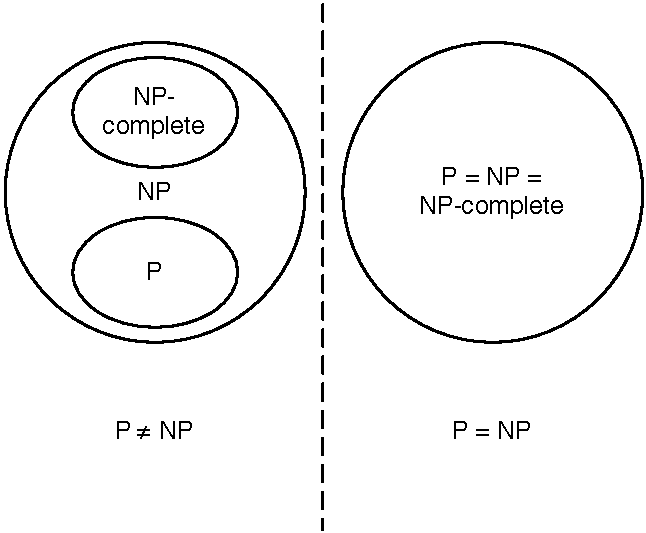
\includegraphics[width=0.4\textwidth]{p=np}
\par\end{center}


\subsubsection{The P versus NP question}

There are two possibilities: either $P=NP$ or $P\neq NP$. So far
we have been unable to prove the existence of a single language in
NP that is not in P. (which would prove they are different). At the
same time we still have not found polynomial time algorithms for all
problems in NP. (which will prove they are the same).

The best method known for solving languages in NP deterministically
uses exponential time. In other words, we can prove that $NP\subseteq EXPTIME$
where $EXPTIME=\bigcup_{k}TIME\left(2^{n^{k}}\right)$, that is the
class of languages that are decidable in exponential time on a single-tape
deterministic Turing machine. Again, this is the practical method
but NP could be contained in a smaller deterministic time complexity
class as we will show in section \ref{sub:Relationship-to-other}.


\subsubsection{Facts:}
\begin{itemize}
\item If $B$ is NP-complete and $B\leq_{P}C$ and $C\in NP$ then $C$
is NP-complete. (Which means that if we want to demonstrate that a
problem is NP-complete we need to show that a known NP-complete problem
reduces to out problem in polynomial time!)
\item $SAT$ is NP-complete (Cook-Levin theorem: very important because
identifies the {}``first'' NP-complete problem) 
\item $SAT\in P\iff P=NP$ (Cook-Levin theorem rephrased)
\item A problem $B$ is NP-hard if and only if there is an NP-complete problem
$A$ that is polynomial time Turing-reducible to $B$. This differs
from NP-complete problems because for those problems there is also
the requirement that $B\in NP$ which is not present here.
\end{itemize}

\subsubsection{Examples of problems in NP-complete}
\begin{itemize}
\item $HAMPATH$ is NP-complete
\item $CLIQUE$ is NP-complete
\end{itemize}

\subsection{Space complexity}

Analogously to what we did for time we estimate space complexity of
Turing machines by using asymptotic notation.

Let $f:\mathcal{N}\rightarrow\mathbb{R}^{+}$be a function. The space
complexity classes $SPACE(f(n))$ and $NSPACE(f(n))$ are defined
as follows.\[
SPACE(f(n))=\{L|L\text{ is a language decided by an }O(f(n))\text{ space deterministic Touring machine}\}\]


\[
NSPACE(f(n))=\{L|L\text{ is a language decided by an }O(f(n))\text{ space nondeterministic Touring machine}\}\]



\paragraph{Savitch's theorem}

For any function $f:\mathcal{N}\rightarrow\mathbb{R}^{+}$, where
$f(n)\geq n$, $NSPACE(f(n))\subseteq SPACE(f^{2}(n))$. This means
that deterministic machines can simulate nondeterministic machines
using a surprisingly small amount of space. Hence the idea that space
appears to be more powerful than time because space can be reused,
whereas time cannot.


\subsection{The class PSPACE and NPSPACE}

By analogy with the class P, we define the class PSPACE as the class
of languages that are decidable in polynomial space time on a deterministic
Turing machine. In other words, \[
PSPACE=\underset{k}{\bigcup}SPACE(n^{k})\]


We define NPSPACE, the nondeterministic counterpart to PSPACE, in
terms of the NSPACE classes. However, $PSPACE=NPSPACE$, by virtue
of Savitch's theorem, because the square root of any polynomial is
still a polynomial.


\subsubsection{Relationship to other complexity classes \label{sub:Relationship-to-other}}

\[
P\subseteq NP\subseteq PSPACE=NSPACE\subseteq EXPTIME\]


The conjecture is that all of these containments are proper. We know
for sure that $P\neq EXPTIME$ which means that at least one containment
is proper, but we don't know which one.

\appendix

\section{Closures}

The following table summarizes the closure properties of language
families with respect to some common operations. 

\begin{tabular}{|c|c|c|c|c|c|}
\hline 
Operation &  & Regular & DCFL & CFL & r.e.\tabularnewline
\hline
\hline 
Union & $L_{1}\cup L_{2}=\{w|w\in L_{1}\vee w\in L_{2}\}$ & Yes & NO & Yes & Yes\tabularnewline
\hline 
Concatenation & $L_{1}\cdot L_{2}=\{w\cdot z|w\in L_{1}\wedge z\in L_{2}\}$ & Yes & NO & Yes & Yes\tabularnewline
\hline 
Star & $L_{1}^{*}=\{\varepsilon\}\cup\{w\in L_{1}\wedge z\in L_{1}^{*}\}$ & Yes & NO & Yes & Yes\tabularnewline
\hline 
Intersection & $L_{1}\cap L_{2}=\{w|w\in L_{1}\wedge w\in L_{2}\}$ & Yes & NO & NO & Yes\tabularnewline
\hline 
Complement & $\overline{L_{1}}=\{w|w\notin L_{1}\}$ & Yes & Yes & NO & NO\tabularnewline
\hline 
Reverse & $L_{1}^{R}=\{w^{R}|w\in L_{1}\}$ & Yes & NO & Yes & Yes\tabularnewline
\hline 
Intersec. with reg. lang. & $L_{1}\cap R=\{w|w\in L_{1}\wedge w\in R,R\,\text{regular}\}$ & Yes & Yes & Yes & Yes\tabularnewline
\hline
\end{tabular}
\begin{itemize}
\item Regular = Regular languages
\item DCFL = Determininistic Context Free Languages
\item CFL = Context Free Languages
\item r.e. = Recursively Enumerable languages
\end{itemize}

\end{document}
